\documentclass{sig-alternate-10pt}

\newcommand{\ttt}{\texttt}

\usepackage{graphicx}
\usepackage{changepage}
\usepackage{lipsum}
\usepackage{booktabs}
\usepackage{booktabs}

\title{FLASH\\Fast Linux Advanced Scheduler Hardware}
\author{
	Mark Aligbe \\
	    \email{ma2799@columbia.edu}
	\and
    Chae Jubb \\
        \email{ecj2122@columbia.edu}
}
\date{4 May 2015}

\begin{document}
\maketitle

\begin{abstract}
As accelerators become more common and necessary as a way to continue
Moore's Law in the absence of Dennard Scaling, researchers explore segments
of computation that can be improved with the aid of dedicated hardware. This
paper presents FLASH, a hardware scheduler, to take over the task of
scheduling from the operating system. FLASH differs from previous hardware
schedulers by implementing a time sharing algorithm, as opposed to
a deadline based or real-time scheduling algorithm. The scheduling decisions
it makes are equivalent to those made in common desktop operating system
schedulers, but in much reduced time and without negatively impacting
processor performance features. FLASH is designed to keep kernel
modifications minimal, only requiring change when the kernel scheduling
interface changes. We discuss the implementation status of FLASH,
work that remains to be done and future work, and its relevance in different computing
platforms.

\end{abstract}


\section{Introduction}
\label{sec:intro}
Desktop operating systems are interactive, meaning that they present
a responsive and fluid experience to users. To achieve this balance of
performance and responsiveness, desktop operating systems are called
preemptable, meaning that the execution of processes can be interrupted by
another process. By contrast, server operating systems are batch oriented,
meaning that processes are not preempted: a process continues until it exits
or is forced to exit, at which point another process starts computation.
This preemption is one of the performance factors that contribute to greater
CPU utilization on server operating systems as opposed to desktop operating
systems. The reason why preemption is detrimental to CPU utilization is
a combination of a few different reasons.

\subsection{TLB and Cache}
The translation lookaside buffer (TLB) is a hardware structure that assists
the memory management unit (MMU) of the CPU in translating virtual addresses
into physical addresses. The TLB serves as a cache to look up commonly used
virtual addresses and returns the corresponding physical address. In
computationally expensive portions of code, this unit is advantageous as it
prevents unnecessary page lookups when the code is accessing small regions
of memory. Likewise, the cache on a CPU provides good speedups to these
kinds of programs by holding the actual data referenced in these virtual
memory locations.

These structures have been shown to work very well, despite their small
sizes. However whenever another task takes residence in the processor, the
cache and TLB are likely invalidated, thus leading to a period of degraded
performance. A context switch is the process wherein the operating system
saves the state of the currently executing task and schedules in a new task
to execute. In order to make a decision on which task is selected next,
a scheduler is invoked. Depending on the needs of the particular operating
system, this scheduler can be a simple queue or a complex multi-queue
priority based scheduler. If the scheduler is sufficiently complex, even if
it chooses the same task to resume running, it may already invalidate the
cache and TLB of the processor. The new resident process must now wait for
expensive memory accesses to bring in valid TLB entries and cache values.
This results in less than ideal processor utilization.

It is also difficult to make real time scheduling guarantees. In applications such as video or audio playback, it is necessary that the playback process be scheduled consistently to ensure jitter-free playback \cite{groves2009bfs}. Schedulers typically run periodically in an operating system to ensure interactivity. If they run too infrequently, a video processing task may not obtain enough cycles to produce a consistent amount of frames. If they run too frequently, then they consume too many system resources and negatively impact scheduling. FLASH is able to solve this conflicting requirement. Since it is a dedicated hardware unit, FLASH does not consume any CPU resources. Additionally, since its decision making is time bounded, it can make real-time scheduling guarantees.

\subsection{Raw Throughput}
In our research, we focus on scheduling in the Linux kernel. In order to determine the limits of the improvements that FLASH can bring, we performed benchmarking based on the CFS scheduler, which we talk more about in Section \ref{sec:sched_in_kernel}. In order to determine the overhead incurred due to the CFS scheduler, we ran the \verb|hackbench| scheduler stress test \cite{hackbench}. \verb|hackbench| operates by launching a large number of threads or processes and passing data between them. In order to measure the amount of CPU time spent in the scheduler subsystem, \verb|oprofile| was used to profile the entire Linux kernel \cite{oprofile}.

Our testing environment consisted of an Intel \textsuperscript{\textregistered} Core \textsuperscript{TM} i7-4810MQ processor, operating at 3.25 GHz. We ran \verb|operf| with the \verb|-k| and \verb|--system-wide| options, before launching \verb|hackbench| with the \verb|-l 100000| option, to ensure that the benchmark ran for a sufficiently long amount of time. The process of starting \verb|operf| and \verb|hackbench| was repeated three times to reduce variability, and the average of the three runs was taken. To obtain the results, \verb|opreport| was run with the following options: \verb|--merge all| \verb|--symbols| \verb|--image-path| \verb|-l| \verb|-e| \verb|sync_buffer,|\verb|add_event_entry,|\verb|dd_sample_entry|.

Finally, we filtered out irrelevant results by searching for entries with fair in their name, and identified the class scheduler functions, as shown in Table \ref{tab:cfs_usage}.

\begin{table}[h]
\begin{center}
	\begin{tabular}{@{}ll@{}}
		\toprule
		CPU Time (\%)      & Symbol Name                    \\ \midrule
		0.8200             & update\_cfs\_shares            \\
		0.0515             & update\_cfs\_rq\_blocked\_load \\
		0.0509             & check\_cfs\_rq\_runtime        \\
		0.2811             & pick\_next\_task\_fair         \\
		0.2670             & enqueue\_task\_fair            \\
		0.2197             & dequeue\_task\_fair            \\
		0.1866             & select\_task\_rq\_fair         \\
		0.0919             & task\_waking\_fair             \\
		0.0077             & idle\_enter\_fair              \\
		0.0071             & migrate\_task\_rq\_fair        \\
		0.0034             & put\_prev\_task\_fair          \\
		9.9e-05            & task\_tick\_fair               \\
		5.8e-06            & task\_move\_group\_fair        \\
		\textbf{1.9870048} & \textbf{Total}                 \\ \bottomrule
	\end{tabular}
	\caption{The CPU usage of the various functions used by CFS to accomplish its task.}
	\label{tab:cfs_usage}
\end{center}
\end{table}

Overall, just 1.99\% of CPU time was devoted to the CFS scheduler. While this may seem like a negligible amount of time, the CPU presented 8 logical cores for scheduling and operated at 3.25 GHz, equating to:
\begin{equation*}
	3.25\ \text{GHz}*0.0199*8 = 508.7\ \text{MHz}
\end{equation*}

We see that $508.7$ million cycles are wasted each second. FLASH is intended
to return many, if not most, of those cycles back to the CPU to perform
useful work.

\section{Scheduling in the Kernel}
\label{sec:sched_in_kernel}
% Mark
Modern desktop operating systems have to run hundreds of tasks, while providing a responsive interface to the user. This means that the CPU must be able to serve many interrupts a second from various hardware devices and service dozens or even hundreds of background tasks while presenting a lag-less experience to the end user. Each of these sources introduces potential sources of latency. Interrupt handling \cite{regehr2007safe} requires many techniques, in both hardware and software implementations, to maintain relatively cheap. Efficient scheduler design is an ongoing field of research \cite{wong2008cfs, park2008hardware, morton2004hardware}. We chose to focus on scheduling for our research as the potential benefits of scheduling in hardware in an operating system are not explored in the context of a desktop workload.

\subsection{History of Linux Schedulers}
The Linux scheduler has gone through some major design changes in its scheduler. Before the introduction of the $ O(n) $ scheduler in Linux 2.4, scheduler implementations as simple and fast as CPUs themselves had not become complex compared to modern CPUs with simultaneous multi-threading (SMT) and symmetric multi-processing (SMP). These implementations were not scalable to multiple processors, so the $ O(n) $ scheduler was introduced to solve these problems. The $ O(n) $ scheduler worked well as long as the number of tasks remained low, but, as it had a single runqueue for all CPUs in a system, scaled poorly as the number of CPUs and processes grew (since it must iterate through the list of all processes to select a candidate).

The $ O(1) $ scheduler was introduced to solve the problem of a large number of tasks. As the name implies, it is able to select a task to run in constant time. The $ O(1) $ scheduler achieves this efficiency by exploiting per-priority \textit{active} and \textit{expired} arrays for tasks. Tasks that are eligible to run are placed in the \textit{active} array and once a task has completed running it is placed in the \textit{expired} array. Thus, selecting a task is as fast as retrieving the head of the highest priority array. Once the \textit{active} array is empty, the \textit{active} and \emph{expired} arrays are swapped by simply changing pointer directions. Unlike the $ O(n) $ processor, it had per-CPU runqueues, meaning task scheduling did not stall other CPUs.
The $ O(1) $ was effective at its job, but was not a fair scheduler; was difficult to maintain through major kernel revisions; and used heuristics to determine the interactivity of a process in a flawed way. The CFS scheduler was introduced in Linux 2.6 as a replacement to solve the interactivity issues of the $ O(1) $ scheduler and introduce a simpler yet efficient scheduler.

\subsection{Implementation of CFS}

\begin{figure}
	\begin{center}
		%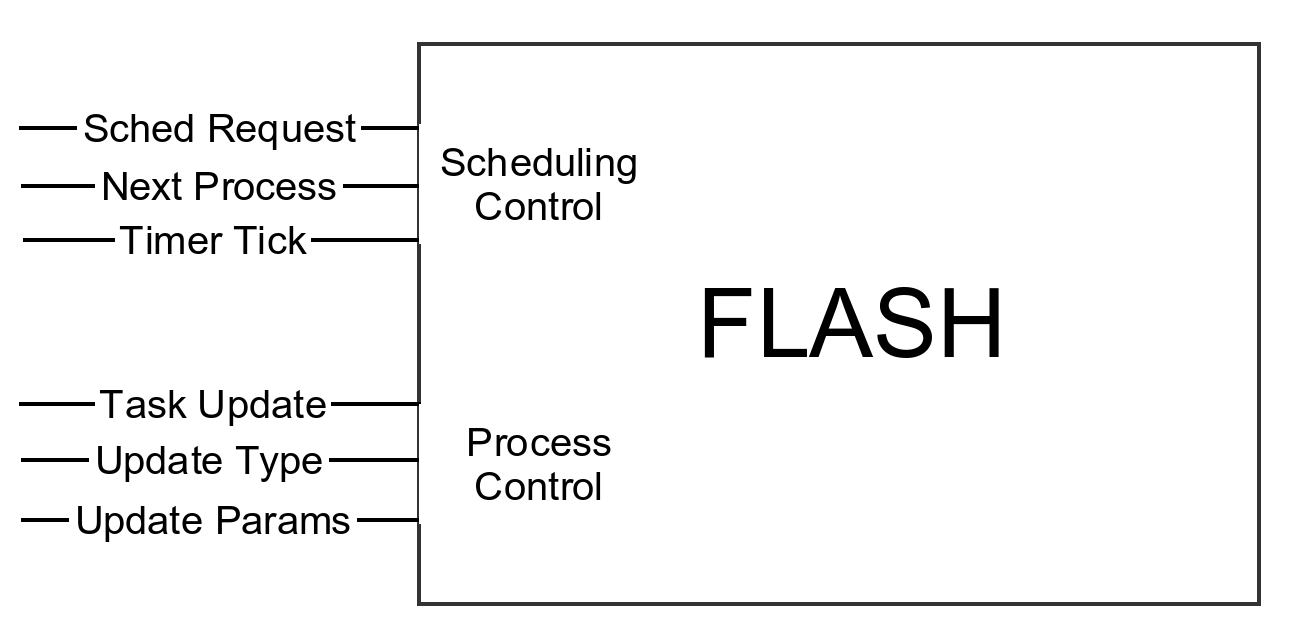
\includegraphics[width=0.65\textwidth]{fig/flash-diagram.png}
		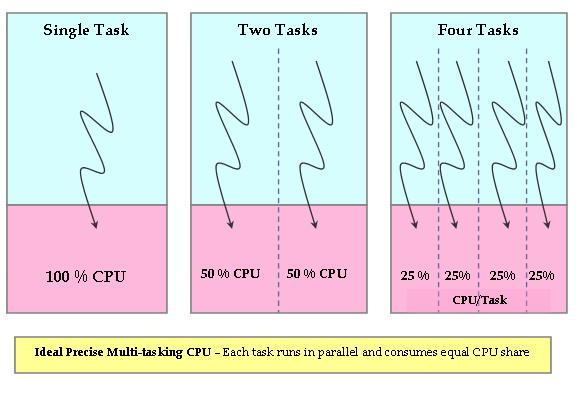
\includegraphics[width=0.9\linewidth]{fig/mutlitasking.jpg}
		\caption{
			Ideal multi-tasking. Taken from \protect\cite{fig:multitask}. Every task gets an equal share of CPU time.
		}
		\label{fig:cfs_multitask}
	\end{center}
\end{figure}

The CFS scheduler is conceptually simple; it aims to implement an ideal
multi-tasking CPU \cite{cfsdesign}. An ideal mutli-tasking CPU assigns equal
time to all processes assigned to it, essentially a restatement of
round-robin scheduling \ref{fig:cfs_multitask}. As \emph{expired} and
\emph{active} arrays are the basis of the $ O(1) $ scheduler, red black
trees are the basis of CFS. Red black trees are a type of self balancing
binary search tree, and, in the case of CFS, ordered based on the virtual
runtime of processes, as defined by the number of nanoseconds in CPU
residence (weighted by task priority). This type of accounting affords CFS
greater granularity than the other process schedulers, as it has no notion
of a timeslice. Instead, CFS simply chooses the task with the smallest total
runtime (with the weighting applied for priority) and schedules it to be run
next. This allows CFS to emulate a round-robin scheduler while offering
greater granularity. Additionally, CFS is conceptually simpler and has
a much smaller code footprint---better for embedded environments, than the
$ O(1) $ scheduler.

\begin{figure}
	\begin{center}
		%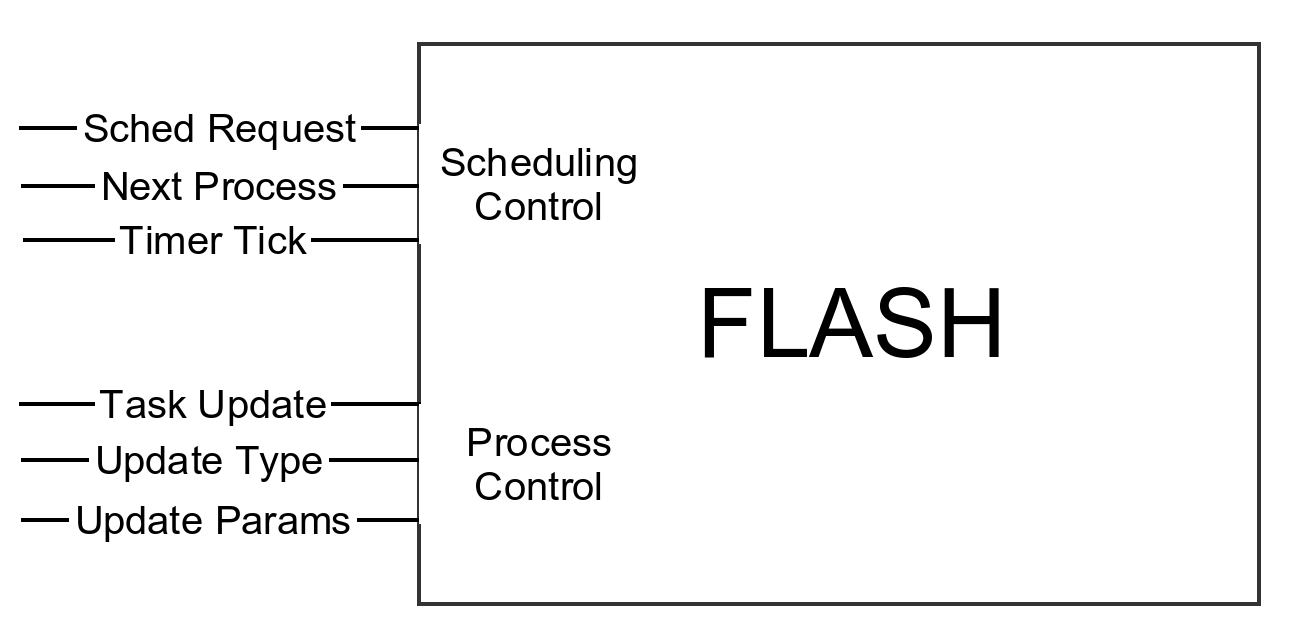
\includegraphics[width=0.65\textwidth]{fig/flash-diagram.png}
		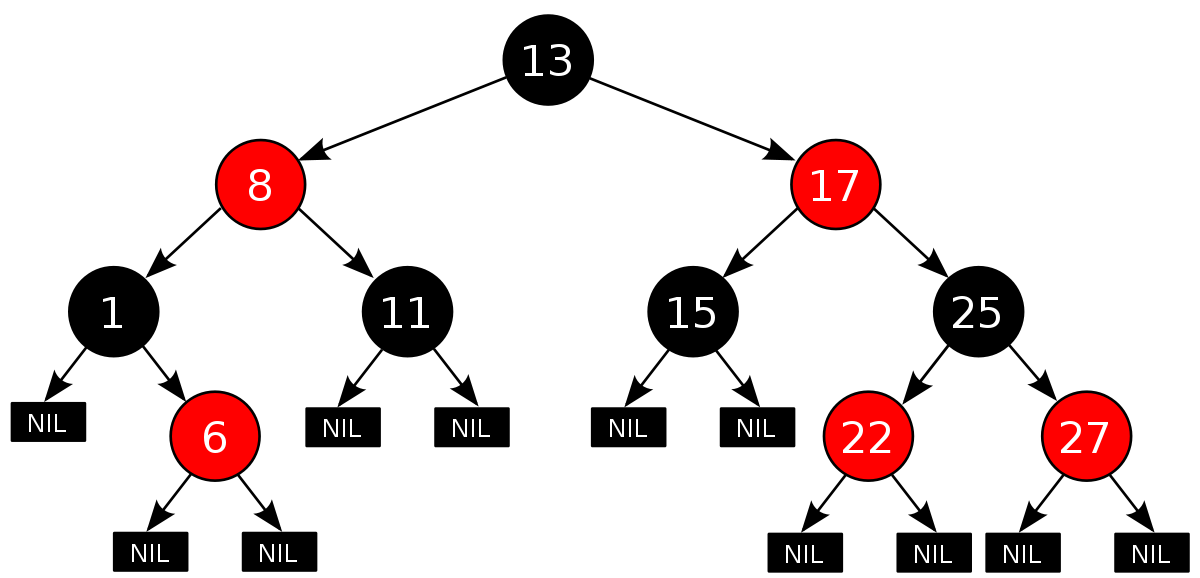
\includegraphics[width=0.9\linewidth]{fig/rbtree.png}
		\caption{
			A sample red black tree taken fron \protect\cite{wiki:rbtree}. The choice of color is arbitrary, and the distinction is used to maintain the balancing property of the tree.
		}
		\label{fig:rbtree}
	\end{center}
\end{figure}

\subsubsection{Limitations}
CFS operates at $ O\left(\log n\right) $ efficiency (inserting
a task back into the red black tree), which is less efficient than the
$ O(1) $ scheduler, but CFS achieves fairness by virtue of its
implementation, without favoring any particular kind of task (e.g.
interactive vs. non-interactive).

\section{Related Works}
\label{sec:related_works}
Previous hardware scheduling units focus completely on embedded systems with
a fixed number of tasks each with fixed priority
\cite{kuacharoen2003configurable, morton2004hardware, nacul2007hardware,
nakano1995hardware, park2008hardware}.  Scheduling under these fairly
restrictive constraints is greatly simplified with respect to desktop
scheduling as the desktop scheduler is much more defined ordering between
tasks.

Additionally, there are often a small number of tasks relative to a desktop
environment.  This means that much simpler algorithms may be used in an
attempt to approximate the optimal task ordering.

The major novel challenge in escalating to a desktop Linux is handling the
dynamic, unbounded (from a realistic hardware perspective) number of tasks.
The initial FLASH prototype addresses this in an unsatisfying way: by
arbitrarily fixing the number of tasks that can be managed with its
scheduling policy.  As discussed in detail in Section~\ref{sec:future},
future iterations will remove this restriction by reserving a small section
of memory.

Because we aim to support an unbounded number of tasks, we must implement
a scheduler comparable to the default CFS scheduler.
While a simpler implementation than the kernel default, the FLASH scheduler
is implemented in accordance with the major principles of CFS
\cite{wong2008cfs}.

We should also consider the architecture of previous hardware schedulers.
Many of the previously cited works were designed either as ASICs
(Application Specific Integrated Circuits) or on FPGAs (Field Programmable
Gate Arrays) rather than a general purpose CPUs.  This makes resource
allocation and scheduling slightly different in that there is not always an
overhead of a context switch: we may simply be deciding which process can
use a particular multiplier.


\section{FLASH Architecture}
\label{sec:arch}
% Chae
The FLASH hardware unit is built with intention of seamlessly replacing the default software implementation. A major addition we add over a standard
scheduler is the ability for the scheduler itself to raise an
interrupt to indicate a tick when it has already computed the result. Either at this tick or when a process is
requested, FLASH will provide the process ID of the task to the run next.
Figure~\ref{fig:arch_overview} gives an overview of the system architecture.

\begin{figure}
	\begin{center}
		%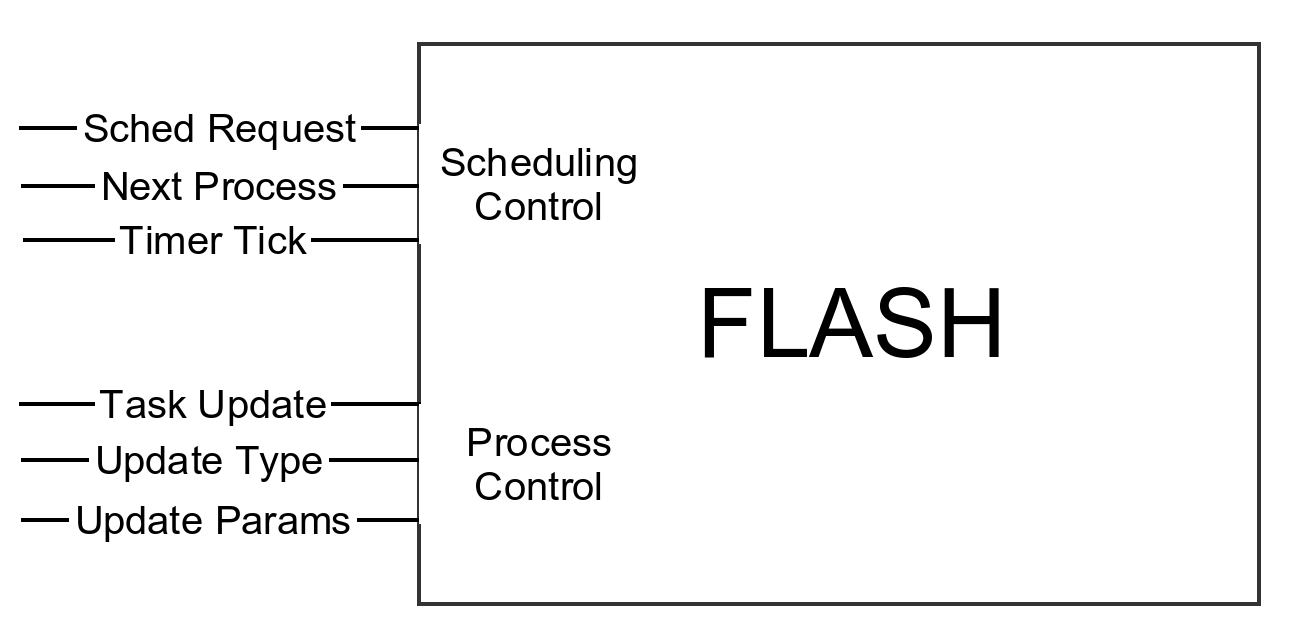
\includegraphics[width=0.65\textwidth]{fig/flash-diagram.png}
		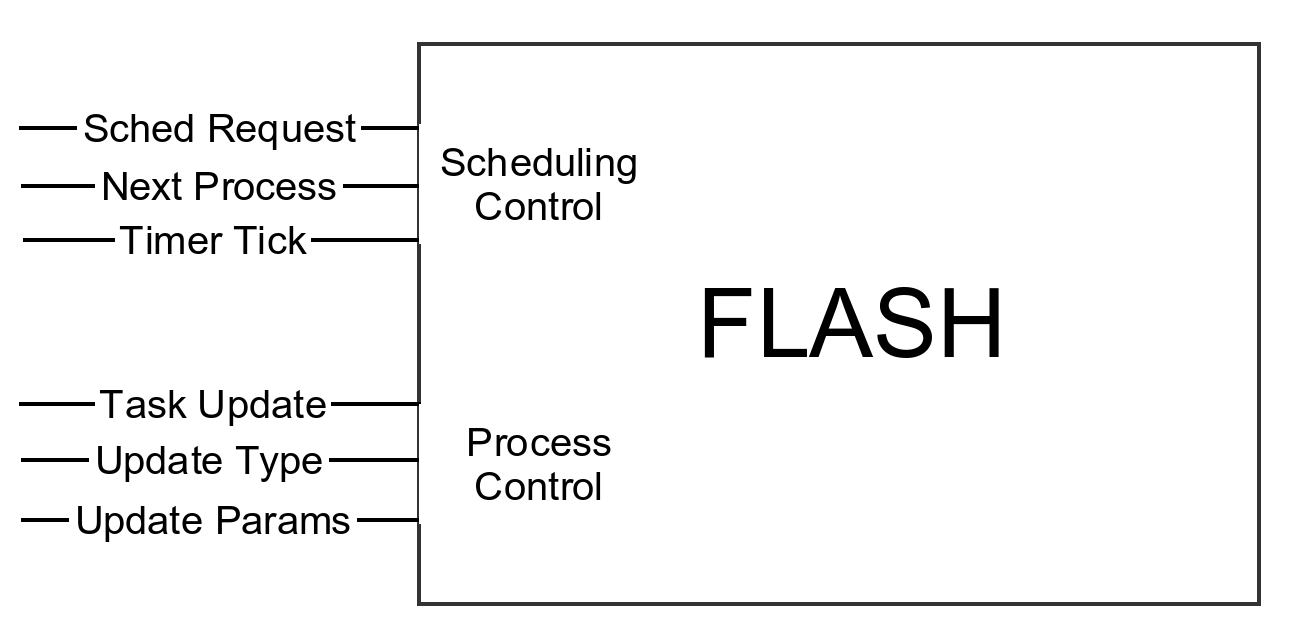
\includegraphics[width=0.9\linewidth]{fig/flash-diagram.png}
		\caption{
			FLASH System Architecture: Interface.  Note the distinction between
			the \emph{Process Control} and \emph{Scheduling Control} Interfaces.
		}
		\label{fig:arch_overview}
	\end{center}
\end{figure}

\subsection{Improvements}
FLASH provides improvements over the CFS scheduler. The most
notable potential advantage is in speed. Having a separate hardware unit
allows the CPU to be running tasks at the same time the choice of next task
is being prepared.  This way the next task can be immediately read without having to
wait for a computation.

Additionally, data structures are maintained in a separate memory structure.  This
means that scheduling computations will not pollute the usual cache
hierarchy or TLB of a processor.  As cache misses are costly, eliminating a small class of
them will directly correlate to a performance increase.  This will be
especially true as modern processor hardware (newer versions of x86 and ARM)
have more effective TLBs that are not, for example, completely flushed on
a context switch \cite{neiger2006intel}.

Increasingly, desktop machines are being used as virtualization platforms.
The problem of TLB hit rate is especially relevant with the added number of
virtual memory spaces so it is important that the TLB stay as intact as
possible through context switches.

\subsection{Scheduling Algorithm}
As previously mentioned, in order to best schedule the set of eligible
tasks, we use the same fundamental algorithm to which the Linux kernel
defaults: the Completely Fair Scheduler.

The kernel's implementation
fundamentally relies upon red-black trees. However, implementing a red-black tree in hardware with a fixed amount of
memory would be prohibitively expensive.  For this reason, the FLASH
implementation utilizes a simple unordered array.  Because there are
typically few tasks eligible to run, the cost of keeping and constantly reorganizing an
ordered data structure would outweigh the cost of a simple iteration.
Further, we must importantly note that this lookup in hardware will be much
quicker than in software, given that the data is stored in a single
monolithic, low-latency memory.  Even more convincing is the ease with which
parallelization of lookup can be implemented using hardware.

FLASH does, however, retain the core functionality of CFS's basic algorithm.
Scheduling decisions are made using the notion of virtual runtime.   Just as
in the Linux implementation, virtual runtime is calculated as a weighted
physical runtime based upon the priority of the task.  FLASH uses the same
relative weighting as CFS.

We now describe in more detail both the interface and internal
implementation of the scheduling unit.

\subsection{FLASH Interface}
At its most basic, the hardware interface is given by two major segments:
\emph{scheduling control} and \emph{process control}.  Together these two
segments allow processes to be scheduled based on an up-to-date accounting
of process status, kept via the process control interface.  The scheduling
controller interface sends timer tick interrupts and serves incoming
requests for new processes to run.

\subsubsection{Process Control Interface}
Let us first focus deeply on this process control interface.  It is here
that FLASH is given information on the state of all running
processes.  Currently, we store process id (PID), priority, and state
triples as passed through the interface using a standard four-phase
handshake.

\paragraph{Consistency} A major hurdle with offloading scheduling decisions
to a dedicated piece of hardware is ensuring consistency between the data
structures maintained by the software kernel and the
hardware unit.

We cannot completely offload the data about processes to hardware, most
obviously because of the size of objects like the \ttt{task\_struct}.
Additionally, those objects are heavily accessed by modules other than the
scheduler.  We must, though, retain some structure in FLASH memory so that
it may make scheduling decisions comparable to that of CFS.

For this reason, we expect each update in process priority or state to be
communicated to FLASH so it may continue making accurate scheduling
decisions.

\subsubsection{Scheduling Control Interface}
In addition to the process control interface, FLASH provides a scheduling
control interface, responsible for providing the software with tasks to be
run.  We can further subdivide this interface into two subparts: scheduling
requests and timer ticks.  Making replacement of software more
straightforward, these subparts directly correspond to the two main mechanisms by which tasks switch in the Linux Kernel.

\paragraph{Scheduling Requests}
Often a running process will want to do something (such as disk I/O) that
requires yielding the processor.  When this occurs, the Linux kernel will
call \texttt{schedule()}.  We modify this function to interact with our
scheduling control interface---more specifically the portion dealing with
scheduling requests.

A scheduling request will be received using a standard four-phase handshake.
At this point, using methods explained in Section~\ref{sec:FLASH_impl}, the
next task to be run is selected and returned to the software.

\paragraph{Timer Tick}
FLASH also provides functionality to raise an interrupts as a way of implementing timer ticks.
For simplicity and fully encapsulating scheduling logic, we export the
generation of the timer tick to this hardware unit.  At a specified time
interval, FLASH will raise a timer interrupt and provide the software with
the next task to be run.

\subsection{FLASH Implementation}
\label{sec:FLASH_impl}
FLASH implements a simplified version of the CFS scheduling algorithm, allowing transparent
replacement of the current software implementation.  Internally, we have two
front-end ports, each corresponding to a segment of the interface (process
control and scheduling control). Those front-end modules connect to back-end
modules which regulate and control access to the backing internal data
structures.  We see this internal implementation architecture described in
Figure~\ref{fig:impl_overview}.

\begin{figure*}
	\begin{center}
		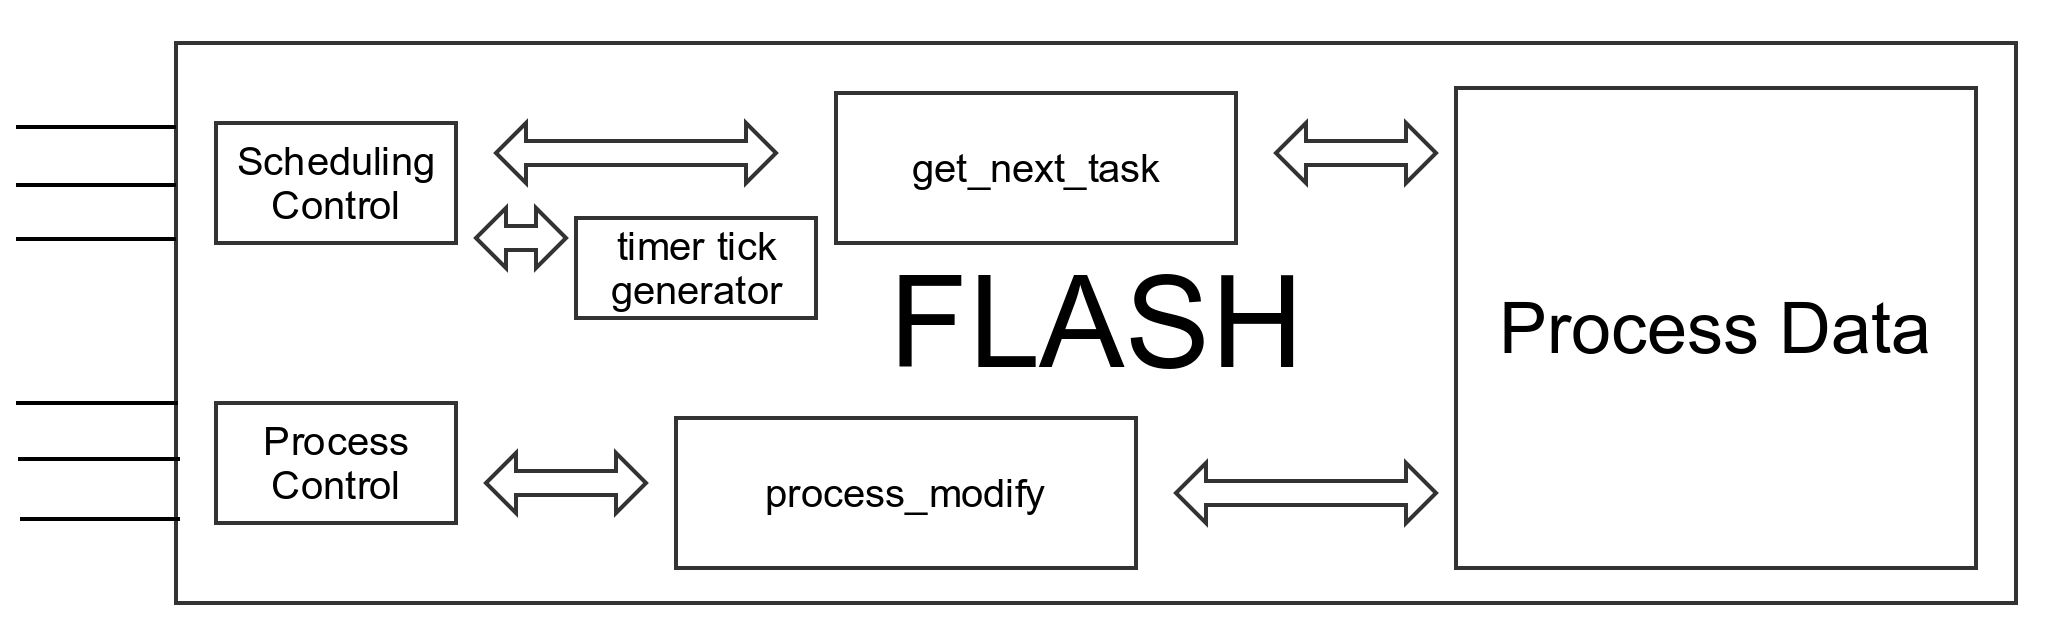
\includegraphics[width=0.9\textwidth]{fig/flash-impl.png}
		%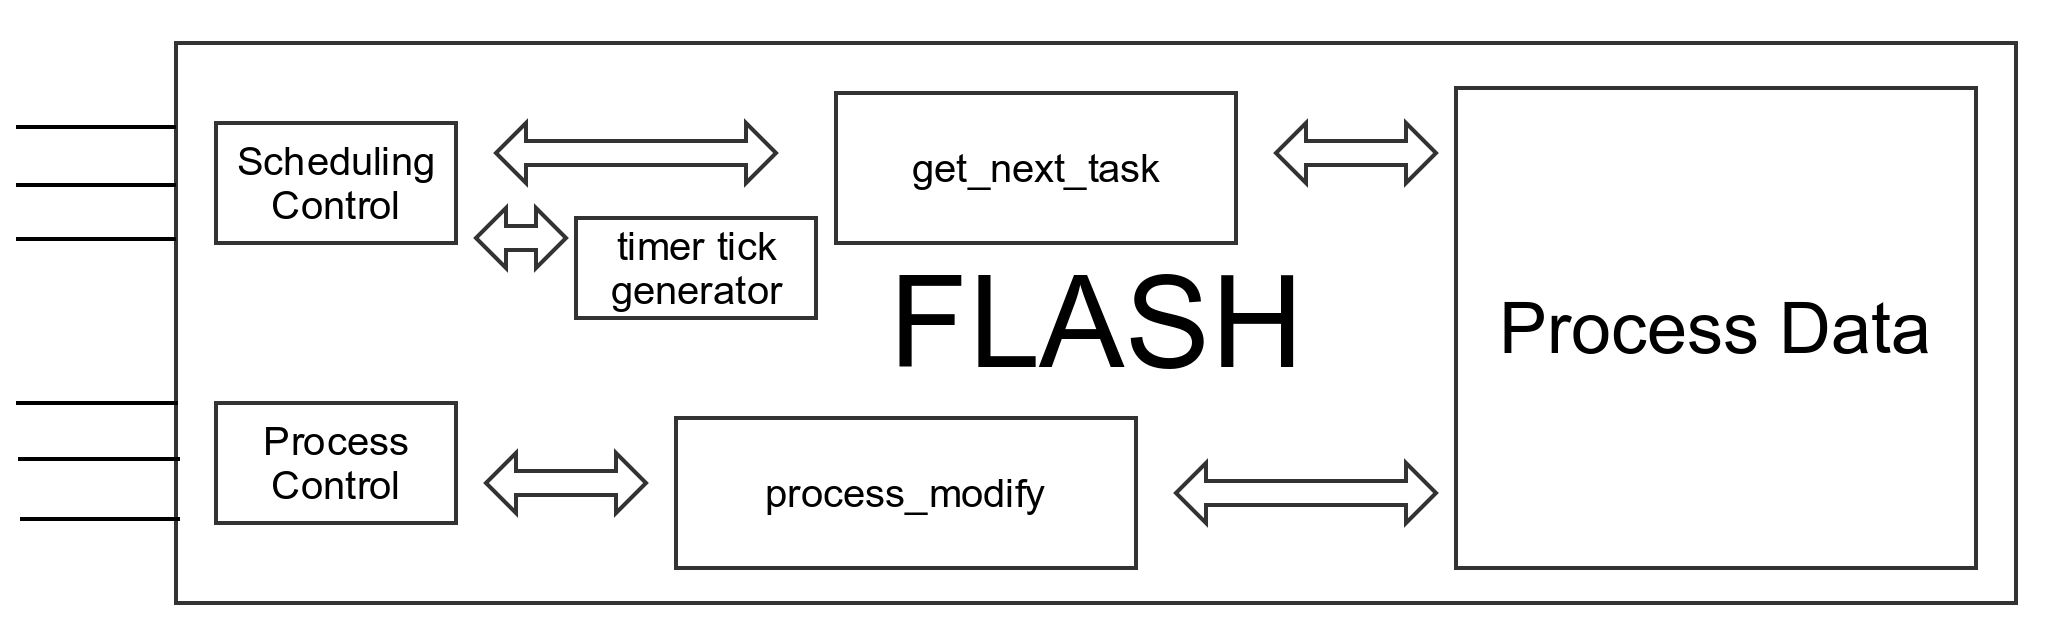
\includegraphics[width=0.9\linewidth]{fig/flash-impl.png}
		\caption{
			FLASH System Architecture: Implementation.  Notice the division
			between the front-end, back-end, and process data modules.  This
			allows tightly regulated access to backing process data store.
		}
		\label{fig:impl_overview}
	\end{center}
\end{figure*}

\subsubsection{Front-End Modules}
As mentioned above, we have a front-end module for each segment of the
interface.  Each of these modules is quite simple.  The module corresponding
to the scheduling control interface has two jobs: responding to scheduling requests
as well as passing on timer ticks generated by a different internal module.
Both of these require querying for the next task to be run.

The second front-end module corresponds to the process control interface.
It will simply communicate through the incoming request and update the
backing store of process state.

\subsubsection{Back-End Modules}
The FLASH back-end modules serve to regulate access to the backing data
store.  This is done via two modules: a reading module and a writing module.
The process control datapath is connected through the writing module as this
interface is used only to modify the state of processes.

Additionally, we have a simple reading module connected to the scheduling
control interface.  This regulates reads to the backing data store in order
to determine the next process that ought to be run.

\subsubsection{Storing Process State}
The current FLASH implementation is a basic version of CFS.  We do not use
the same type of implementation as the Linux kernel because implementing
red-black trees in hardware would be prohibitively complex.  Instead, we use
a simple array.

The FLASH scheduling algorithm, like CFS, will keep record of the runtime of
the process as well as a \emph{virtual runtime}.  This virtual runtime is
a weighted accounting of the actual runtime based on priority of the
process.  Scheduling decisions are made based on the virtual runtime, as in
CFS.  FLASH additionally stores other minor fields for bookkeeping purposes.

\paragraph{On Red-Black Trees}
While using a red-black tree would allow the implementation to be
asymptotically faster, actual runtime in software is likely to be higher than
the number of cycles needed to iterate through a simple queue in hardware.  Firstly, hardware
will simply be faster than software as it is more easily parallelizable.
The hardware can parallelize comparisons in logarithmic time, whereas iteration in software will take linear time.

Secondly, traversing the red-black tree in software will not have ideal cache
performance. Switching to a self-contained hardware module will not have any
cache considerations because that hardware unit will have a single
monolithic memory.

\paragraph{What We Store}
In addition to storing the PID, priority, and state, we also have a few
fields used to store the internal state necessary to keep our CFS implementation
completely fair.  These fields most importantly include a notion of virtual
runtime.  Other fields are for bookkeeping.

\subsection{Summary}
Together the interface and implementation of FLASH provide an easily
integrable scheduling module.  The kernel will interface with the hardware
unit in the same way that the software scheduler does.  Additionally, FLASH
implements the fundamental algorithm of the current default Linux scheduler
CFS, which schedules based on priority-weighted virtual runtimes.


\section{Integration}
\label{sec:integration}
% intro stuff here
\begin{figure}
	\begin{center}
		%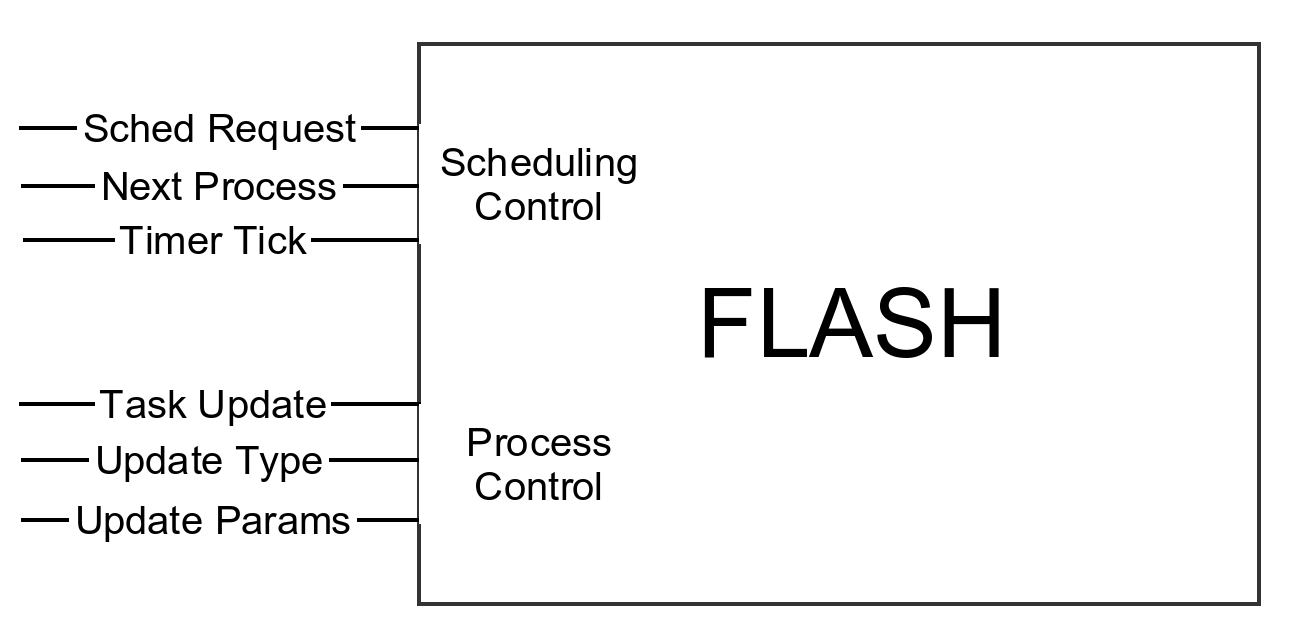
\includegraphics[width=0.65\textwidth]{fig/flash-diagram.png}
		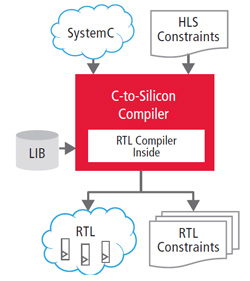
\includegraphics[width=0.9\linewidth]{fig/hlsctos.jpg}
		\caption{
			The SystemC workflow. The design is written using SystemC, and then ``scheduled'', or compiled to RTL using specified design paramteres and the CtoS compiler.
		}
		\label{fig:ctos_overview}
	\end{center}
\end{figure}

In testing FLASH, a platform that enables rapid prototyping is essential.
There are two components to prototyping FLASH; however. The first is the
choice of development language. While the software component must be written
in C, there are many choices for a hardware descriptive language. In order
to quickly iterate on the design of FLASH, a high level hardware descriptive
language was chosen, SystemC. Unlike Verilog and VHDL which specify hardware
at the Register Transfer Level (RTL), SystemC allows designs to
be specified in ``hardware'' aware C/C++. Designs can be written using C/C++
syntax and a basic notion of time flow, but the code style is still oriented
towards hardware limitations, excluding constructs like pointers, dynamic
memory allocation, dynamic stack values, and things generally made possible
by having a large standard library and a large memory bank. We use Cadence
C-to-Silicon (CtoS) to compile our SystemC code to RTL, which is then used
in our second prototyping component.

Since our design is a hybrid between custom hardware and software, we need a device that is capable of being dynamically reconfigured combined with a Linux-capable processor. Such a platform is the Arrow SoCKiT, powered by Altera's Cyclone V.

\subsection{Cyclone V}
% Mark
\begin{figure}
	\begin{center}
		%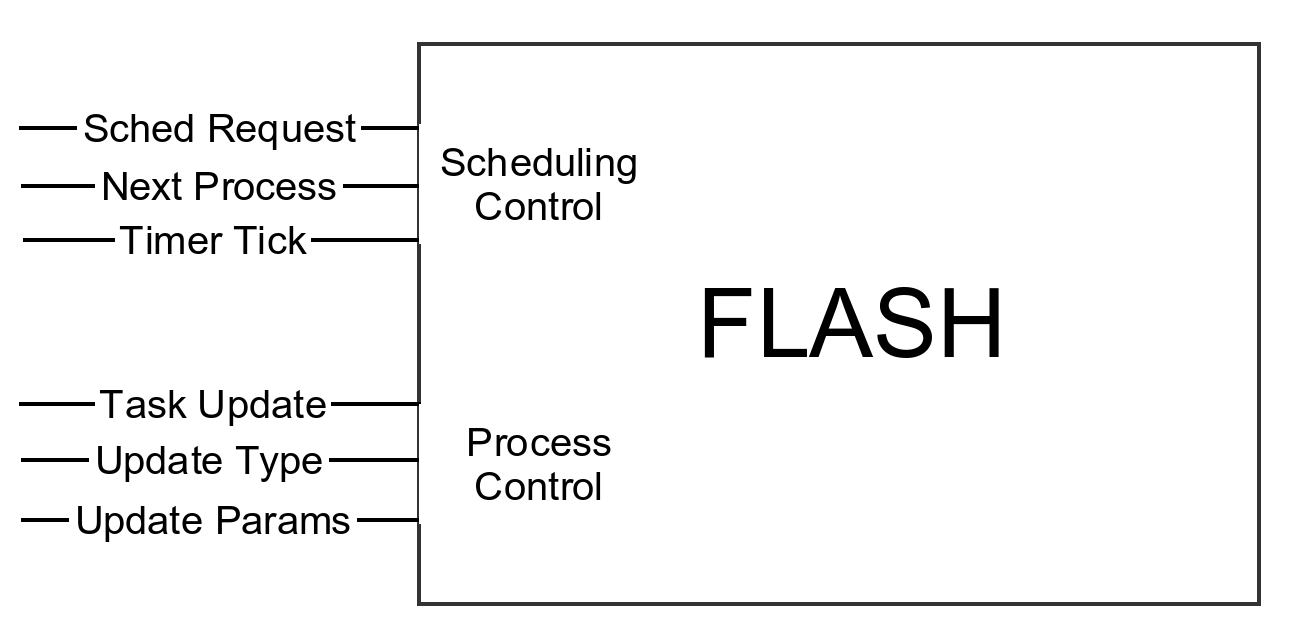
\includegraphics[width=0.65\textwidth]{fig/flash-diagram.png}
		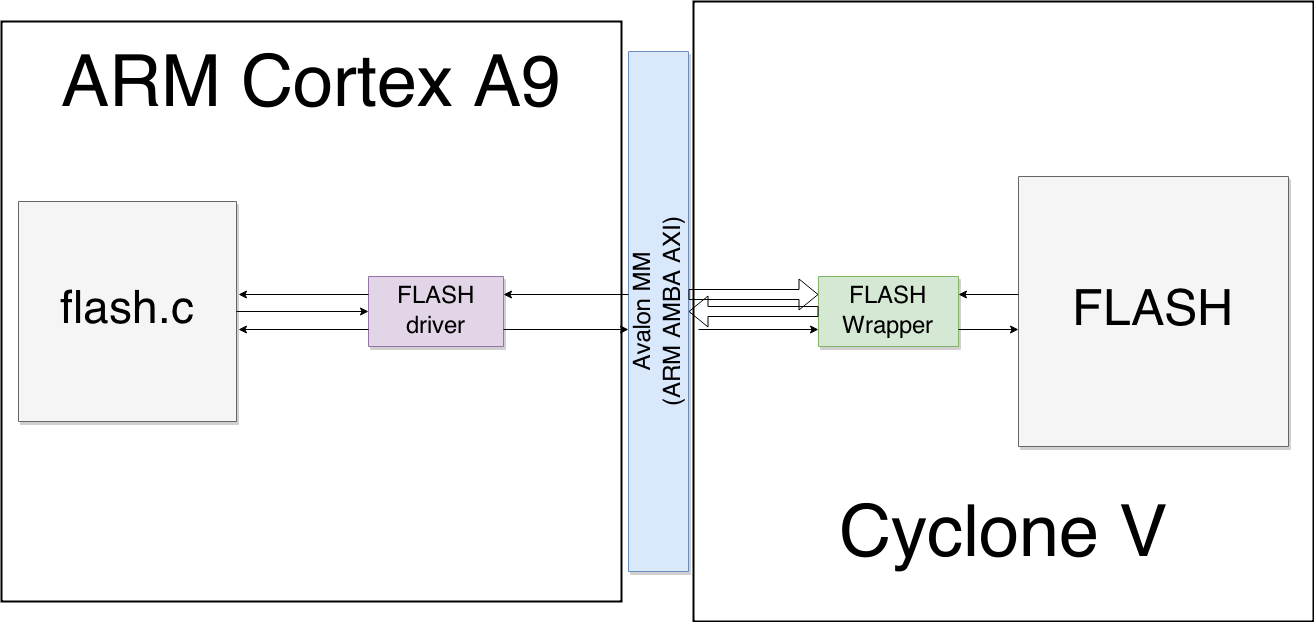
\includegraphics[width=0.9\linewidth]{fig/sockit-architecture.png}
		\caption{
			Arrow SoCKiT high level overview. The embedded ARM processor is connected to the FPGA fabric via a ARM's AMBA AXI interface, on top of which runs Altera's Avalon MM interface.
		}
		\label{fig:sockit_overview}
	\end{center}
\end{figure}

The Cyclone V family of Field Programmable Gate Arrays (FPGA) also includes
System on Chip (SoC) configurations. In these configurations, the FPGA is
connected to a hard processor system (HPS) realized by an ARM Cortex A9, as
shown in Figure~\ref{fig:sockit_overview}.

\subsubsection{Quartus}
The first step in realizing our design is synthesizing the design using Altera Quartus II. Quartus is Altera's IDE for designing and verifying RTL descriptions targeted at their FPGAs. Once the design is compiled to RTL using CtoS, it is then configured in Quartus using Qsys, which is a system integration tool also developed by Altera that facilitates the task of connection complex modules to complex systems. In order to communicate with the HPS, hardware modules are connected to the Avalon MM bus which is implemented on top of ARM's AMBA AXI interface for communication with the ARM processor. Once the design is connected using Qsys, it is synthesized using Quartus, and then a bitstream used to program the FPGA is generated.

\subsubsection{U-Boot and Kernel}
\begin{figure}
	\begin{center}
		%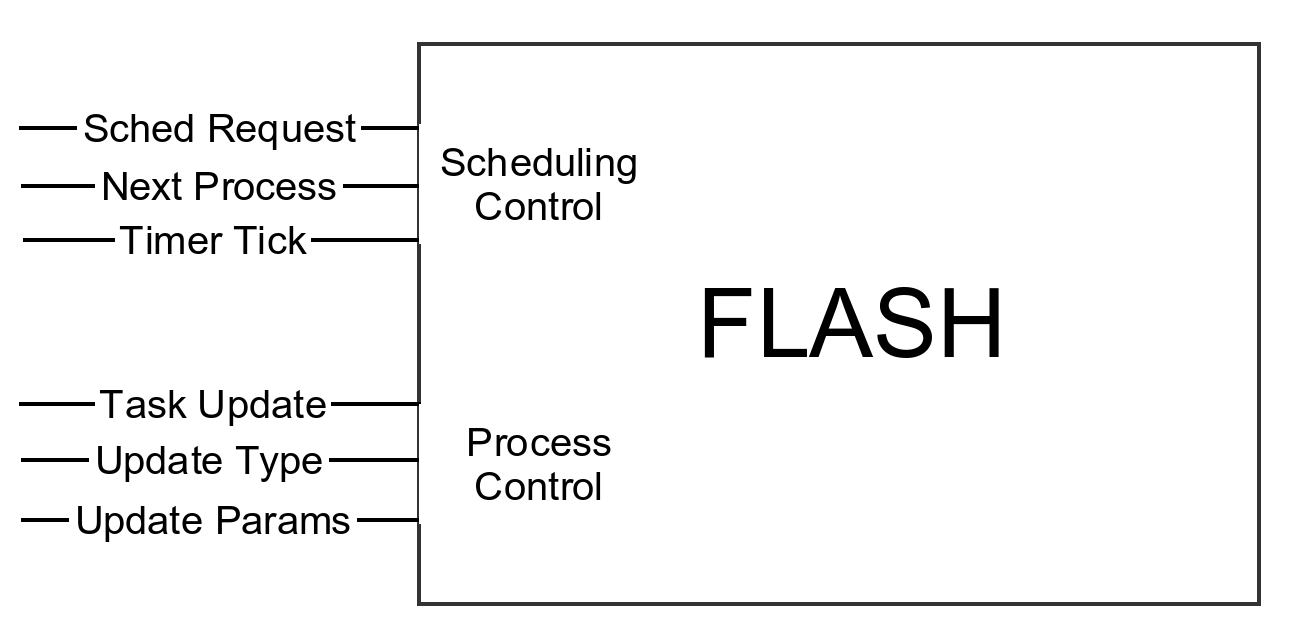
\includegraphics[width=0.65\textwidth]{fig/flash-diagram.png}
		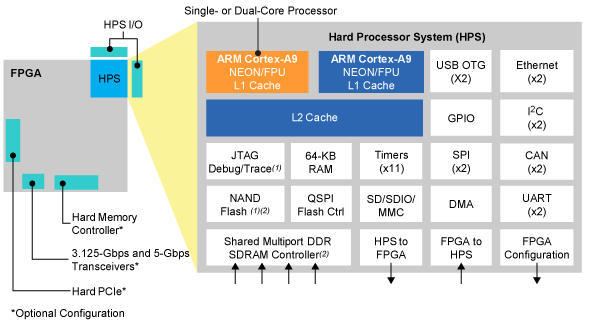
\includegraphics[width=0.9\linewidth]{fig/soc_cyclonev.png}
		\caption{
			Arrow SoCKiT high level overview. The embedded ARM processor is connected to the FPGA fabric via a ARM's AMBA AXI interface, on top of which runs Altera's Avalon MM interface.
		}
		\label{fig:cyclone_diag}
	\end{center}
\end{figure}

U-Boot is a bootloader targeted for embedded devices, similar to GRUB for
desktop Linux computers. U-Boot differs from GRUB in that its boot parameters
are included in the generated binary for the target device, specifying the
location of the kernel image and a special file called the Device Tree Blob
(DTB). The DTB is essentially a binary form of the Device Tree Source (DTS),
which specifies all the hardware available to the processor on the embedded
device, and their address location and size. Support for generating device
tree blobs is part of the kernel \cite{dts_Linux}, and provides a simple
mechanism for embedded developers to make their hardware available to the
associated processor. We use the dts for the Cyclone V provided by
RocketBoard.org, who provide Linux sources and tools for various embedded
devices, and modify it to include the ``lightweight bus'', or the Avalon MM
interface, and specify the address of our ``flash'' device.

The kernel image is cross built using the GCC ARM~v7 toolchain, using the
sources from rocketboards.org configured for the Cyclone V SoCKiT. These
sources contain branches for a variety of SoC devices as well as
configurations for accessing their hardware, with the Cyclone V layout shown
in Figure \ref{fig:cyclone_diag}. Then, to boot Linux on the SoC, the SoCKiT
must be configured to boot from the appropriate source, either over ethernet
using BOOTP or as in our case, from a micro SD card. The U-Boot image is
used to bootstrap the Linux kernel \emph{uImage} also located on that same
source. 

\subsubsection{Ubuntu Linaro}
\label{subsubsec:linaro}
However, a root filesystem still needs to be provided. There are two main choices; a Buildroot distribution, which is a distribution targeted specifically for embedded devices. We will talk more about Buildroot in Section \ref{sec:eng_exp}. The option we chose was Ubuntu Linaro, a distribution of Ubuntu targeted for ARM devices. Since the Cyclone V contains a relatively powerful ARM processor, it is capable of running a full desktop Linux distribution backed by the micro SD card. We use this as our basis of evaluation to determine the relevance of FLASH in a practical device such as a smartphone or Chromebook. The Ubuntu Linaro distribution also has access to a larger collection of software, such as Xorg and gcc, both of which are critical to evaluation. The Linaro distribution can be downloaded as an archive containing the entire root filesystem, and then extracted to whichever source the kernel will be booted from.

\subsection{Kernel Modifications}
% Chae
In order to actually take advantage of our custom hardware, we need to
inform the operating system---here, Linux---that the new device is available
to be used.  This requires creating a device driver to communicate with the
device, and, additionally, a Linux scheduling class and policy to use it as
a scheduler.

\subsubsection{FLASH Device Driver}
The primary purpose of the FLASH device driver is to facilitate
communication between the Linux kernel and the FLASH hardware device.
Because the possible types of communication are quite limited, the device
driver is fairly simple.  The kernel either asks for a task to schedule or
provides an update about process status.  In the opposite direction, the
device only provides the next tasks to be run as well as raising an
occasional interrupt.

Upon initialization, the driver will register the device and then allocate
a memory region to be used as internal device registers.  Finally, we must
register an interrupt handler to handle the interrupt generated by the
device upon each timer tick.

Once the device has been initialized, the driver will simply serve requests
(as instructed by the scheduling policy) via a series of \texttt{iowrite32}
and \texttt{ioread32} function calls.  This will come in addition to
handling device-generated interrupts and passing them up through the stack.

Device destruction is simply the reverse of device initialization.  When the
device is in the destroyed state, the FLASH scheduling policy may not be
used as reads from and writes to the device will fail.

\subsubsection{FLASH Scheduling Policy}
Now that we have constructed a device driver and can communicate with the
FLASH device, we must implement a scheduling policy that allows us to use
the novel device as a scheduler.

Implementation of this policy is done using the usual scheduling interface
provided by the Linux kernel.  We construct a \texttt{struct sched\_class}
and the implementation of the relevant core scheduling functions such as
\texttt{enqueue\_task}, \texttt{dequeue\_task}.  We implement the provided
interface in a way that is a thin wrapper around calls to device driver
functions.  This is because the algorithmic work is done in the device, so
we need only relay decisions made by the device to the core scheduler.

After the scheduling class has been implemented, we must modify the core
scheduler itself to make FLASH the default scheduling policy.  This way all
tasks will be scheduled using the FLASH policy unless explicitly specified
otherwise.  As we are implementing a replacement scheduler for CFS, we place
our scheduling policy at a higher priority than CFS.  However, we keep it
below policies such as real-time.

\paragraph{Scheduling Policy Priorities}
The available scheduling classes in the Linux kernel are kept in
a prioritized linked list.  Here priority refers to the ordering in which
scheduling policies will be asked for tasks to run next.  A higher
priority policy, such as real-time, will always be able to run a task if it
has one in the runnable state, even if lower priority policies such as idle
have multiple tasks in the runnable state.

\subsubsection{Kernel space Interface}
To further abstract the implementation of the scheduling policy, a pleasant
interface is provided to the user were they to use standard kernel
functions to control the behavior of the scheduler in a non-default way.
This includes updating process priority or state of those processes on the
FLASH scheduling policy.  A \texttt{struct} with these relevant fields is
provided so that only the driver need worry about the bit ordering that the
device itself expects to receive.  This interface, for example, would
provide users of both little endian and big endian a generic interface in
a similar way the socket API provides functions such as \texttt{htonl} and
\texttt{ntohs}.


\section{Applications}
\label{sec:apps}
% Mark
Our intention in developing FLASH was to produce a device that would ultimately find adoption in heterogeneous computing platforms (like the Apple ``A Series''), where specialized function cores are used to accelerate the function of a CPU. We also believe that our device can be relevant as an accelerator unit in modern monolithic CPUs.

\subsection{MMU-like Device}
\label{subsec:mmu}
The Memory Management Unit is a fundamental part of all processors with
large amounts of RAM. Its task is to keep accesses to virtual memory fast
and correct and to alleviate many of the memory performance issues
associated with multi-tasking operating systems and large address spaces.
Without the MMU, the virtual memory abstraction provided by operating
systems would result in multiple accesses for each memory access a program
makes. The Translation Lookaside Buffer (TLB) is the core of the MMU and its
task is to cache a fixed number of virtual memory translations. The size of
the cache depends on the hardware. For the Cortex A9, the TLB contains up to
4 by 32 entries, resulting in at least 8192 bits of storage (assuming 32 bit
addresses) \cite{arm_mmu}.

The information for the total number of gates an MMU requires in a given CPU architecture is not very forthcoming, but the factor that normally dominates a design size is the memory usage. Our design by comparison uses 8.5 kb of storage, which is directly comparable to the memory usage of the Cortex A9 MMU.

\subsection{Obstacles to Adoption}
The main reason why the MMU is present on any desktop operating system
processor is that its performance boost is crucial to keeping these devices
running fast, as explained in Section~\ref{subsec:mmu}. There are two
improvements FLASH could potentially bring, and need to be proven in order
for any sort of adoption to take place, one feature that must be further
researched, which we talk about in Section~\ref{subsec:flash_size}, and
a final aspect which must be addressed.

\subsubsection{Performance}
The first improvement is performance improvements; as the MMU makes memory
access fast, FLASH must also make scheduling fast. The
minimum acceptable speed likely depends on the target workload.  It may be
permissible if FLASH is not much faster so long as it provides significant
energy efficiency over computing in software. Naturally, slower CPUs will
take longer to make a scheduling decision.  However, FLASH operates on a 50
MHz clock.  This means with 50,000 cycles to make a scheduling decision,
FLASH can make scheduling decisions at approximately 1 kHz. Thus, FLASH is
less sensitive to processor speed than processors are in the context of
making scheduling decisions. For this reason, we believe that low power
systems would be ideal candidates for FLASH adoption.

\subsubsection{Energy Savings}
Some low power systems (like smartphones) are as complex, if not more so,
than laptops and desktops. In the case of smartphones and tablets, many contain
dedicated Intellectual Property cores (IP) that perform certain tasks, like
network management, video acceleration, USB communication, and so on. These IP
cores typically free up the CPU from performing a processing intensive task
that it either cannot perform (Wi-Fi communication) or would be tedious (SPI
communication). We believe that FLASH can benefit such a system. FLASH would
free up the CPU on smartphones to service the interrupts it constantly
receives instead of repeating the mundane task of scheduling the many
background tasks that run on these devices.

\subsubsection{Infinite Tasks}
Since FLASH is a hardware construct, it has a finite amount of memory. Thus,
it can only support a fixed maximum number of tasks. Since threads are also
schedulable entities, this maximum number can be reached relatively easily
on a desktop Linux environment. Thus, it will be necessary for FLASH to
maintain structures in main memory in order to support an unbounded number
of tasks.  This might involve evicting tasks that have a long runtime and
are less likely to continue running in the future.


\section{Engineering Experiences}
\label{sec:eng_exp}
% both
The road to Ubuntu Linaro on the SoCKiT with a communicable FLASH device was fraught with many hardships. We discuss the work done leading up to this development.
% \lipsum[1-3]
\subsection{DE2}
Our initial testing environment was the Terasic DE2, an FPGA development board powered by Altera's Cyclone II. It differs greatly from the Cyclone V in that it does not come with a hard processor system; instead one instantiates a NIOS II processor using Altera's tools. The problem was that the combination of the DE2 and the NIOS II processor was prohibitive to building custom kernels.

There were two main problems: booting a custom kernel and developing a NIOS
II system. Our first attempt at running Linux on the DE2 was successful
using precompiled images, but we would need to modify the kernel and system
to add FLASH. Rather than modifying both at the same time, it would be more
prudent to modify one at a time and verify that the system still functions.
Attempts to build a custom kernel were successful, but booting the kernel
was a separate matter. There were simply too many configuration items to
inspect, and the documentation and tutorial for doing so all relies on
repositories that are no longer in service.

In trying to synthesize a NIOS II system, one immediate issue was that all
instruction resources but one relied on the SOPC Builder, which is the precursor to
Qsys. As none of the authors had experience with SOPC Builder, we used the
Qsys approach, but were stalled by yet another file to be retrieved from
a decommissioned repository. Attempts to regenerate the file and substitute
it in the relevant commands yielded results that were not workable.
Ultimately, the age of the DE2 was prohibitive to using it as our testbed,
and thus we transitioned to the more modern SoCKiT towards the end of our
research.

\subsection{Buildroot}
Buildroot, as briefly discussed in Section~\ref{subsubsec:linaro}, is a root
filesystem for an embedded device. Building and installing Buildroot was
relatively straightforward. However, when it came to developing software on
the device itself to speed up testing, Buildroot's package selection was lacking. In
addition to lacking Xorg, it also had some routing issues that were
prohibitive to getting the package manager to work. Additionally, the
package manager did not seem to operate correctly as attempts to use any
functions other than its help were met with blank output and a zero exit
status. While it was simpler to build than Linaro, it was simply not
functional and not representative of a true desktop Linux distribution.

\subsection{Acts of God}
One of this paper's authors experienced a few severe technical difficulties
over the course of research. The largest incidents occurred in mid March and
early April, essentially costing this author three weeks of productivity.
The incident in mid March was the malfunction of this author's last
functioning laptop, at which point the author decided it would be prudent to
correct his other malfunctioning laptops so that a similar situation would
not arise in the future. The incident in early April was the theft of all of
the author's laptops, which had recently all been made functional. The
author has come to appreciate that anti-theft software is a good investment,
and the author has also learned that it is important to synchronize one's
work environment across all of one's available development machines.

\subsection{CtoS and RTL}
As previously mentioned, this undertaking used high level synthesis (HLS)
tools.  In order to use this design, we must synthesize onto the Altera
board.  This is traditionally done using Altera's proprietary Quartus suite
of software.  Thus, we need to bridge the gap between the HLS-ready SystemC
and RTL that can ultimately be synthesized.  In order to do this, we rely
upon Cadence's C-to-Silicon (CtoS) compiler.  However, CtoS requires that we
plug into a synthesis tool such as Quartus in order to perform area and
timing analysis for the design and construction of local memory blocks.

This process, however, was not straightforward.  Because CtoS only supports
using the subscription version of Quartus and authors did not have enough
institutional clout to have this expensive license installed on the same
server as the CtoS tool, the authors were forced to complete this
compilation to RTL using Quartus' main competitor: Xilinx's Integrated
Synthesis Environment (ISE).  This resulted in some non-optimized synthesis.

Overall, the experience of using CtoS was pleasant, especially as it allowed
some design-space exploration, making some area vs. timing tradeoffs.
Because our design only pushed the area capacity of the board with a high
static task limit, most optimizations erred on the side of timing in order
to take full advantage of the board's speed.  There was some trouble
integrating these disjoint toolchains, but with a proper environment setup,
many of these problems would likely disappear.


\section{Future Work}
\label{sec:future}
While the framework of the FLASH scheduler is complete, it still needs to be tested and evaluated. Due to time constraints, we were not able to reach the evaluation phase. There are also two features that could potential improve the performance of FLASH that are not present in the current implementation.

\subsection{DMA}
\begin{figure}
	\begin{center}
		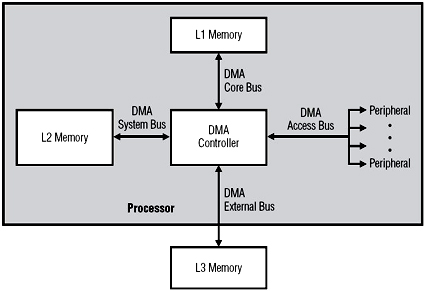
\includegraphics[width=0.9\linewidth]{fig/dma.jpg}
		\caption{
			A block diagram of the function of DMA access, and how it frees up the processor from becoming involved in data transfers \protect\cite{fig:dma}.
		}
		\label{fig:dma_diag}
	\end{center}
\end{figure}
In Direct Memory Access (DMA), a controller handles the task of maintaining
memory coherency with the processor while it is executing, as shown in
\ref{fig:dma_diag}. This overhead is justified because the processor can
continue executing while the controller interfaces with the device to
read/store data. The advantage of DMA in the context of FLASH is that
instead of performing an \texttt{ioread}/\texttt{iowrite} every time a scheduler event occurs,
the processor and device can use the DMA as a liaison and access the data
when they are ready.

This does not negate the necessity of retrieving a new process immediately
if the current process calls \verb|sched_yield|, for example, but it reduces
the number of \texttt{ioread}s/\texttt{iowrite}s when there are plenty of processes in the
running state.

\subsection{No HZ Interrupt}
Desktop Linux kernels use a timer to manage rescheduling needs. The speed of the timer directly corresponds to the interactivity of the kernel, with 1000 Hz yielding the most interactive kernel configuration supported, but with necessarily the poorest throughput. In transitioning to DMA, we can decide whether or not to raise interrupts after FLASH has made a scheduling decision. If our decision is the same as the currently running process, then there's no reason to raise an interrupt. This is another source of a potential performance improvement on tasks like a full kernel build, for example, where there are likely to be few other runnable tasks in the system.

\subsection{FLASH Size}
\label{subsec:flash_size}
In order to tackle the question of how does FLASH stack up to other embedded
CPU accelerators (MMU, memory controller) of similar functionality, we also
need to know the size (area and gate usage) of these components, as well as
FLASH when synthesized for a specific technology node. Unfortunately, the
information of these sizes is not made publically available, and would
likely require us to get in contact with engineers at Intel, AMD, or ARM.

\subsection{SMP Support}
The current implementation of FLASH has no knowledge of multiple processors. This is problematic because only one task can be running at a time from the point of view of FLASH. However, enabling SMP support in FLASH is not as simple as informing FLASH of the number of CPUs; the hardware also needs to be able to make scheduling decisions for each of the processors efficiently. Naturally, this increases the logic usage for the scheduling kernel, but ideally the number of tasks supported in memory need not be increased, thus keeping the memory usage, and potentially area usage, still low and competitive with other CPU units.

\section{Conclusion}
\label{sec:conclusion}
% \lipsum[1]
In this paper, we present FLASH, a hardware scheduler accelerator designed
to replace an operating system scheduler. FLASH performs scheduling
decisions in hardware, thus freeing up the CPU to focus on useful work.
FLASH implements a time-sharing algorithm, which allows for good
interactivity on desktop workloads. Future work for FLASH involves using DMA
to further free up CPU time in combination with interrupts, to reduce the
number of unnecessary scheduler interrupts. Additional future work involves
demonstrating the viability of FLASH in various devices like smartphones as
well as direct, tight integration with CPUs.

\nocite{*}
{
	\bibliographystyle{abbrv}
	\bibliography{ref}
}

\end{document}
